\documentclass[12pt, twoside]{article}
\usepackage{jmlda}
\newcommand{\hdir}{.}

\begin{document}

\title
    [Исследование свойств локальных моделей] % краткое название; не нужно, если полное название влезает в~колонтитул
    {Исследование свойств локальных аппроксимирующих моделей в задаче декодирования сигналов головного мозга}
\author
[] % список авторов (не более трех) для колонтитула; не нужен, если основной список влезает в колонтитул
{} % основной список авторов, выводимый в оглавление
[Филатов А.В., Маркин В.О., Стрижов В.В] % список авторов, выводимый в заголовок; не нужен, если он не отличается от основного
\email
{filatov.av@phystech.edu; markin.vo@phystech.edu}
\organization
{МФТИ}
\abstract
    {
		В данной работе рассматривается проблема создания нейрокомпьютерного интерфейса. Особенностью этой проблемы является требование к устойчивости моделей. Под устойчивостью модели понимается малое изменение выходных данных при малом изменении входных данных. Одним из подходов в задаче декодирования сигнала, удовлетворяющему требованию устойчивости, являются локальные модели. В данной статье рассматривается построение локальной модели на данных электрокортикограммы.
		
		Основной вклад данной работы заключается в  построении локальной модели за счет пространственной информации. В предложенном подходе  пространственная аппроксимация искомого сигнала строится при помощи нормального распределения и полиномов. Параметризация, полученная при помощи локальной модели, рассматривается как новое признаковое пространство для задачи Food-Tracking. В статье приведены результаты численных экспериментов на данных электрокортикограмм головного мозга обезъян.
		
\bigskip
\noindent
\textbf{Ключевые слова}: \emph {отбор признаков; нейрокомпьютерный интерфейс; электрокортикограмма; локальные модели }
}

\maketitle
\section{Введение}
Нейрокомпьютерный интерфейс (Brain-Computer Interface, BCI) \cite{shih2012brain} 
считывает сигналы поверхности кортекс головного мозга, анализирует и переводит в команды исполняющей системы. Исследования в данной области позволяют людям заменить или восстановить нарушенные двигательные функции организма. Примером такой системы является система управления роботизированным протезом посредством мозговых импульсов. 

Мозговая активность~\cite{motrenko2018multi} представляет собой совокупность электрических импульсов различной амплитуды и частоты, возникающих на поверхности кортекса головного мозга. Исследование мозговой активности производится при помощи  электрокортикографии~\cite{hill2012recording} или  электроэнцефалографии~ \cite{aminoff2012electroencephalography}. Результатом измерений является временной ряд напряжений сигнала, который используется в задаче декодирования сигнала. Для исследования используется данные из \cite{chao2010long}.

 Подходы \cite{morishita2014brain, alexander2013traveling} к решению задачи состоят в извлечении информативных признаков из пространственных, частотных и временных характеристик сигнала.В~\cite{chin2007identification, eliseyev2014stable, loza2017unsupervised} исследуются частотные характеристики кортикограмм. Основными методами решения являются линейные модели, такие как метод частичных регрессии наименьших  квадратов (Partial Least Squares, PLS)~\cite{eliseyev2014stable,eliseyev2016penalized, rosipal2005overview} и метод главных компонент (Principal Component Analysis, PCA)~\cite{rosipal2005overview, eliseyev2016penalized}.
 Важным аспектом создания таких моделей является построение надежного
 признакового пространства
  В~\cite{zhao2014coupled} используются алгоритмы, построенные на скрытых марковских моделях. В~\cite{loza2017unsupervised, zhao2010ecog} рассматриваются различные участки сигнала в виде слов. В работе \cite{motrenko2018multi} задача отбора признаков сводится к задаче квадратичного программирования (QuadraticProgramming Feature Selection) \cite{rodriguez2010quadratic}. Также для решения задачи используются нейросетевые модели\cite{xie2018deep}. 
\newpage
\section{Постановка задачи}
\begin{figure}[]
	\centering
  	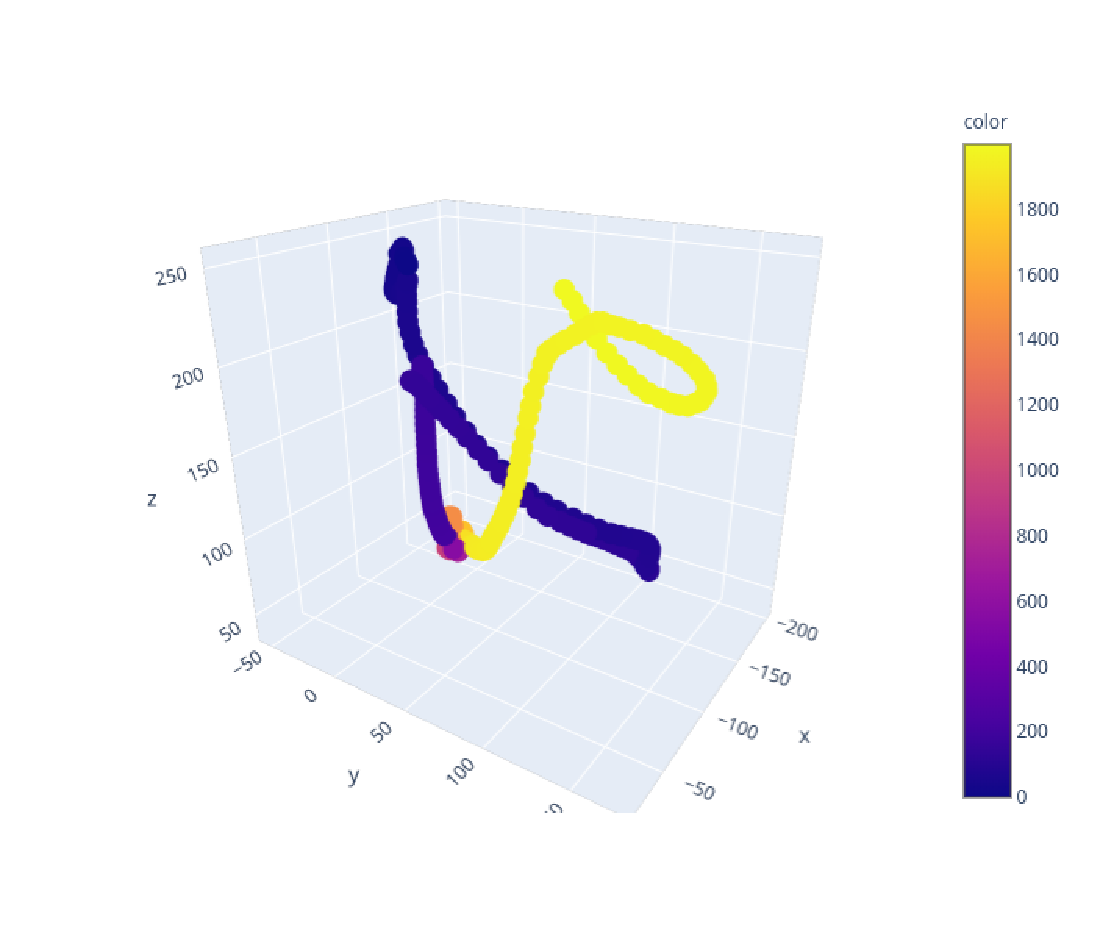
\includegraphics[width=0.5\textwidth]{newplot.pdf}
  	\caption{Пример движения запястья}
\end{figure}

Данные электрокортикограммы представляют собой временной ряд амплитуд сигналов $\mathbf{X}(t)  \in \RR^{m}$, по которым требуется предсказать положение запястья в следующим момент времени $\mathbf{y}(t+1) \in \RR^3$. В качестве выборки рассматривается $\mathfrak{D} = \{(\mathbf{X}_{t}^n, \mathbf{y}_{t+1}\}$, где $\mathbf{X}_{t}^n$ --- значения временнего ряда с момента времени $t$ по момент $t + n$, где $n$ --- горизонт прогнозирования задачи. В силу коррелированности исходных данных предлагается построить предсказательную модель как композицию  локальной модели и линейной модели.

\begin{Def}
	Локальная модель --- совокупность двух параметрических отображений: $\phi$ и $\psi$ 
	\[
	\phi: \RR^{n \times k_1} \rightarrow \RR^{n \times k_2}
	\]
	\[
	\psi: \RR^{n \times k_2} \rightarrow \RR^{n \times k_1}
	\]
	\[
	\psi^*, \phi^* = \argmin_{\psi, \phi} \|\mathbf{X} - \psi \circ \phi (\mathbf{X}) \|_2,
	\]	
	где 
	$\phi$ отображает из пространства большей размерности в пространство меньшей размерности, а $\psi$ отображает из этого же пространства меньшей размерности в исходное пространство большей размерности.
\end{Def}

\begin{Def}
	Под сложностью модели понимается число оптимизируемых параметров.
\end{Def}
\begin{Def}
	Пусть $f$ --- модель, $x, y$ --- произвольные элементы из генеральной совокупности, такие что расстояние $\rho(x,y) < \epsilon$. Тогда модель $f$ называется устойчивой если 
	\[
	\|f(x)- f(y) \| \leqslant C \cdot \epsilon, \text{где $C = \const.$}
	\] 
\end{Def}

Локальная модель порождает новую выборку $\mathfrak{D}_\text{new} = \{(\mathbf{Z}_{(i)}^{n}, \mathbf{y}_i)\}$, $\mathbf{Z}_{(i)}^{n} = \phi(\mathbf{X}_{(i)}^{n})$. На этой выборке строится линейная модель, которая решает конечную задачу:
\[
	\mathbf{w}^* = \argmin_{\mathbf{w}} L(\mathbf{z}, \mathbf{w}, \mathbf{y})
\]

Критерием качества линейной модели выступают коэффициент детерминации и корреляция Пирсона.


\section{Вычислительный эксперимент}
Основная цель --- сравнение моделей результатов моделей с и без использования локальных моделей
\subsection{План работы}
\begin{itemize}
\item Подготовить данные
\item Применить локальную модель к данным
\item Подать выход локальной модели на вход PLS
\item Получить результаты
\item Получить результаты без использования локальной модели 
\item Сравнить результаты
\end{itemize}
\subsection{Данные}
В качестве данных для проведения вычислительного эксперимента использовались данные \cite{chao2010long}, представляющие запись электрокортикограммы головного мозга обезьяны. Каждой записи соответствует амплитуды напряжения на 32 электродах и 3 пространственные координаты.
При проведении эксперимента выборка была сокращена в 10 раз.

\begin{figure}[]
	\centering
	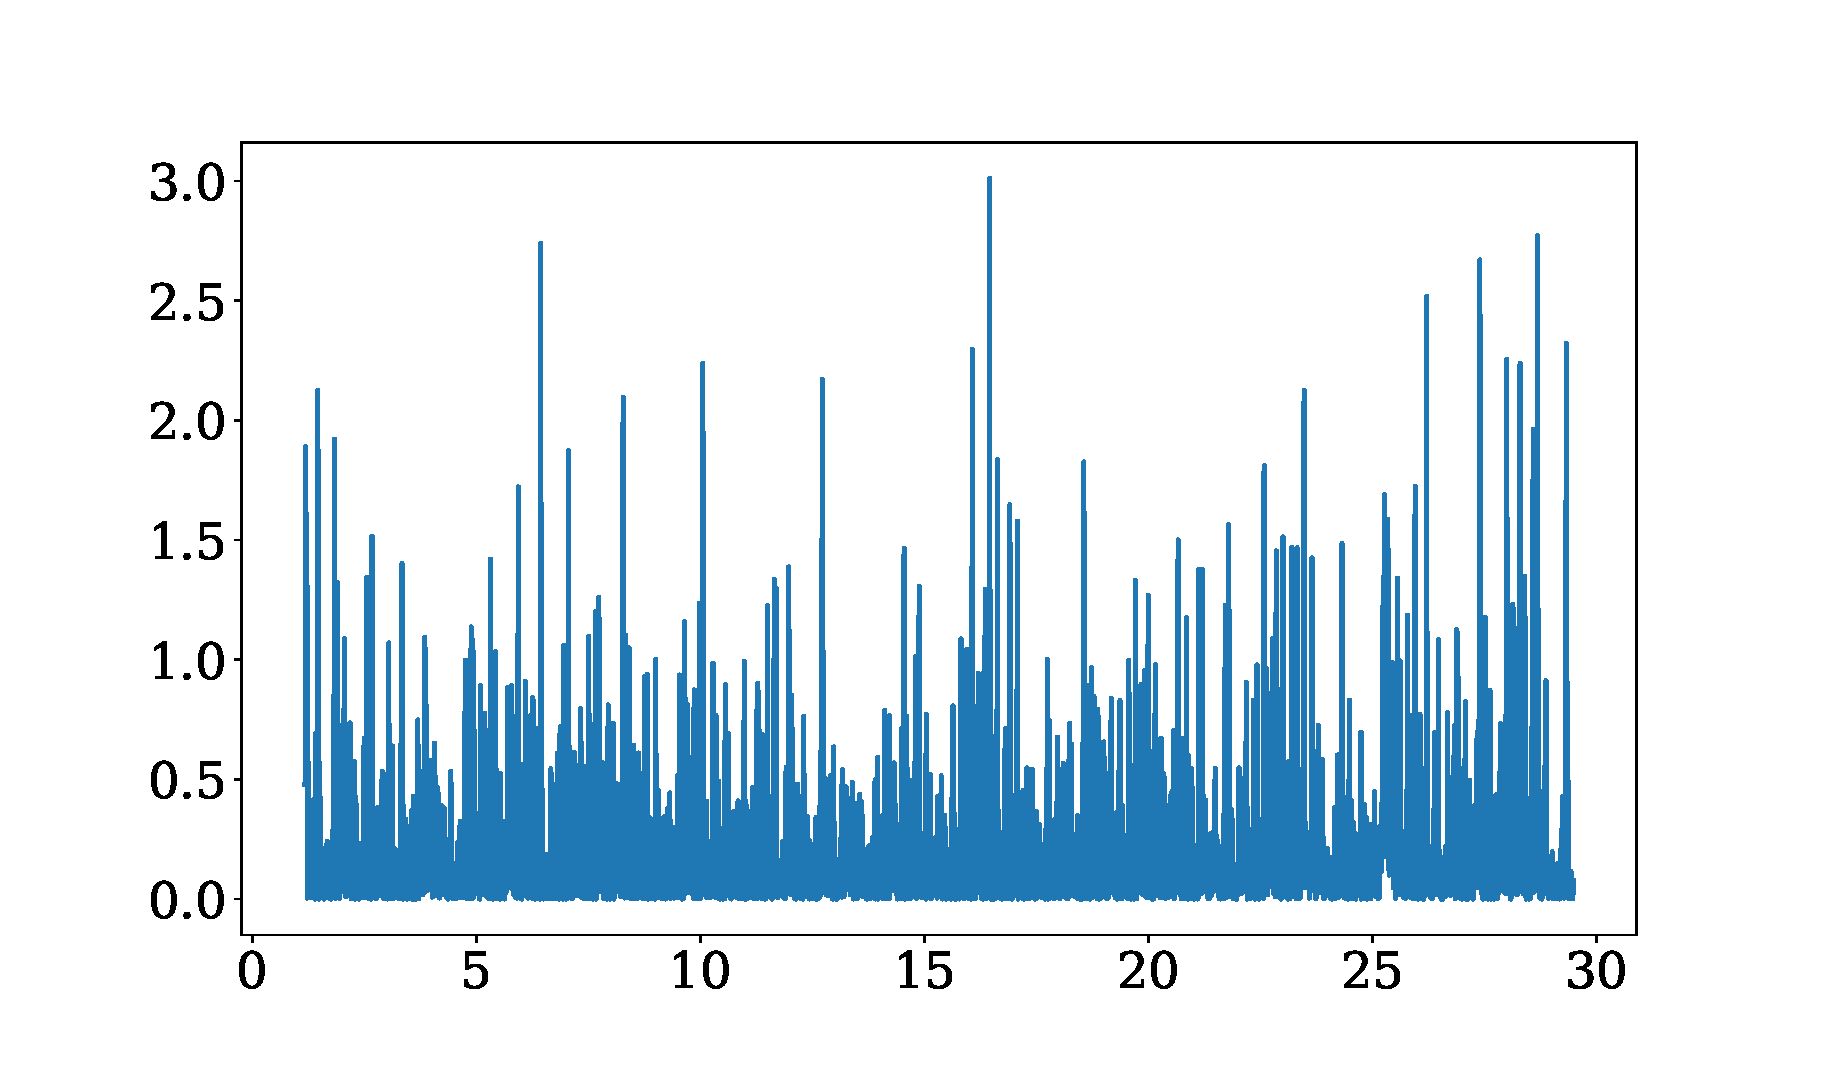
\includegraphics[width=0.5\textwidth]{0freq.eps}
	\caption{Амплитуда сигнала на частоте 10 Гц за первые 30 секунд}
\end{figure}
Обработка исходных данных производится в несколько этапов и подробно описано в статье \cite{zhao2010ecog}. Исходный сигнал записан на частоте $1$ кГц, данные о движении — на частоте $120 $ Гц. Сигнал фильтруется полосным фильтром с диапазоном от $0.3$ до $600 $ Гц. Затем для каждого момента времени $t$ строится частотно-временная
характеристика. Над сигналом в окне $[t - 1.1s, t]$ с шагом в $\Delta$ = $100$ миллисекунд осуществляется вейвлет-преобразование на $10$ различных частотах $\omega_j$ в диапазоне от $10$ до $150$ Гц. Затем строится матрица \mbox{$10 \times 12$}, элементами которой $s_{ij}$ является квадрат амплитуды на частоте $\omega_j$ в момент времени \mbox{$t - (1 + i)\Delta$}. Таким образом, размер описания одного объекта (момента времени) составляет $N_\text{ch} \times 10 \times 12$.

При проведении эксперимента разбиение выборки производится в следующем соотношении: $80\%$ --- обучение, $20\%$ --- тестирование.

\subsection{Алгоритм}
\subsubsection{Локальная модель}
Пусть заданы координаты каждого электрода на плоскости $\mathbf{Z} = \{\mathbf{z}_j \in \RR^2, j \in {1, \ldots N_\text{ch}} \}$. Зафиксируем произвольный момент времени $t$. Тогда представим вектор значений $\mathbf{x}(t)$ амплитуд на электродах в момент $t$, как вектор-функцию $\mathbf{g}(\mathbf{Z})$ от координат электродах. Вектор-функцию $\mathbf{g}(\mathbf{Z})$ ищем в классе полиномов $\{z_{0j}^iz_{1j}^k\}_{i,k = 0}^{n_1, n_2}$, где $z_{0j}$ соответственно первая координата $j$-го электрода, а $n_1$ --- максимальная степень полинома. Находим $\mathbf{g^*}(\mathbf{Z})$ как решение задачи оптимизации:
\[
\mathbf{g^*} = \argmin_{\mathbf{g}} \|\mathbf{x}(t) - \mathbf{g}(\mathbf{Z})\|_2
\]

Отображение $\phi$ строим как: 
\[
	\phi: \mathbf{x}(t) \rightarrow \pmb{\Theta}(t), 
\] где $\pmb{\Theta}$ веса $\mathbf{g^*}(t).$
\subsubsection{Метод частичных квадратов (PLS)}

Метод частичных наименьших квадратов проецирует матрицу плана $\mathbf{X}$ и целевую
 матрицу $\mathbf{Y}$ в скрытое пространство малой размерностью $l$ $(l < M)$. Метод PLS находит в скрытом пространстве матрицы $\mathbf{T}, \mathbf{U} \in \RR
^{m\times l}$, которые лучше всего описывают оригинальные матрицы $\mathbf{X}$ и $\mathbf{Y}$. При этом PLS максимизирует взаимосвязь между $\mathbf{T}$ и $\mathbf{U}$.
Матрица плана $\mathbf{X}$ и целевая матрица $\mathbf{Y}$ проецируются в скрытое пространство следующим образом:
\begin{equation*}
\begin{split}
\underset{m\times n
}{\mathbf{X}}= \underset{m\times l}{\mathbf{T}} \cdot \underset{l\times n
}{\mathbf{P}^T}
+ \underset{m\times n}{\mathbf{B}}
=
\sum_{k=1}^{l}
\underset{m\times 1}{\mathbf{t}_k}
\cdot\underset{1\times n}{\mathbf{p}^T_k}
+ \underset{m\times n}{\mathbf{B}}
, 
\\ 
\underset{m\times r}{\mathbf{Y}}
= \underset{m\times l}{\mathbf{U}} \cdot \underset{l\times r
}{\mathbf{Q}^T}
+ \underset{m\times r
}{\mathbf{C}}= \sum_{k=1}^l
\underset{m\times 1}{\mathbf{u}_k} \cdot \underset{1\times r}{\mathbf{q}^T_k}
+ \underset{m\times r}{\mathbf{C}}.
\end{split}
\end{equation*}

Здесь $\mathbf{T}$ и $\mathbf{U}$ – образы исходных матриц в скрытом пространстве, причём столбцы матрицы
$\mathbf{T}$ ортогональны; $\mathbf{P}$ и $\mathbf{Q}$ – матрицы перехода; $\mathbf{E}$ и $\mathbf{F}$ – матрицы остатков. Метод PLS
максимизирует линейную зависимость между столбцами матриц $\mathbf{T}$ и $\mathbf{U}$
\[\mathbf{U} \approx \mathbf{TB}, \mathbf{B} = diag(\beta_k), \quad \beta_k = \mathbf{u}^T_k 
\mathbf{t}_k/(\mathbf{t}^T_k\mathbf{
t}_k).
\]

Предсказание строится как $\hat{\mathbf{Y}} = \mathbf{XR}$, где $\mathbf{R} = \mathbf{W(P^TW)}^{-1}\mathbf{(T^TT)}^{-1}\mathbf{T^T}$, а $\mathbf{W}$ --- обучаемая матрица весов для поддержания ортогональности.
\subsection{Результаты}

\begin{table}[h!]
	\centering
	\begin{tabular}{|c|c|c|c|}
		\hline
		Метод & $R2$ score & Корреляция Пирсона & Сложность \\ \hline
	Без локальной модели	&                          &                    &           \\ \hline
	Полиномы 3 степени	&                          &                    &           \\ \hline
		&                          &                    &           \\ \hline
	\end{tabular}
\end{table}
\newpage
.
\newpage
\bibliographystyle{unsrt}
\bibliography{references}
\end{document}
